\documentclass[output=paper,draft,draftmode,colorlinks,citecolor=brown]{langscibook}
\ChapterDOI{10.5281/zenodo.7353629}

\author{Elly van Gelderen\affiliation{Arizona State University}}
\title{The Negative Existential and other cycles: Jespersen, Givón, and the copula cycle}
\shorttitlerunninghead{The Negative Existential and other Cycles}


\abstract{\citet{Veselinova2013} provides two sources for negative existential constructions: (a) the univerbation of a negative and a part of the existential construction, which needs not be verbal, and (b) the reanalysis of a lexical item with an appropriate, negative sense. I argue that this definition is both too narrow and too broad when examining the Negative Existential Cycle (NEC). Regarding (a), copulas and auxiliaries provide input to the NEC in addition to existentials, in e.g. \citet{Croft1991}, and regarding (b), verbs with a negative meaning are better seen as a separate development, as in \citet{Givon1978}. I will contend that copulas, auxiliaries, and existential verbs can all fuse with the negative and then disappear into the negative whereas negative verbs,such as \textit{fail,} trade their semantic negative features into grammatical ones without fusion or loss. This paper will address three specific questions relevant to the NEC. The first is what are the source verbs in this cycle. A second question is whether or not the NEC is essentially a verbal cycle, in contrast to the nominal nature of the Jespersen Cycle (JC; \citealt{Jespersen1917}). The third question involves the possible doubling of the negative, which is relevant to showing the NEC is different from the Jespersen Cycle. The role of verbal agreement and inflection sets apart the verbal cycles (NEC and the Givón Cycle) from the nominal one (JC) and the two verbal cycles are different in their renewal. The differences will be shown in their reanalyses in the last section.

\keywords{auxiliary, copula, doubling, existential, negative}
}

\IfFileExists{../localcommands.tex}{
   % add all extra packages you need to load to this file

\usepackage{tabularx,multicol}
\usepackage{url}
\urlstyle{same}

\usepackage{listings}
\lstset{basicstyle=\ttfamily,tabsize=2,breaklines=true}

\usepackage{langsci-optional}
\usepackage{langsci-lgr}
\usepackage{langsci-gb4e}

%from elena-----------------------------------
\usepackage{pgfplots,pgfplotstable}
\definecolor{lsDOIGray}{cmyk}{0,0,0,0.45}
\usepackage{xassoccnt}
\newcounter{realpage}
\DeclareAssociatedCounters{page}{realpage}
\AtBeginDocument{%
  \stepcounter{realpage}
}
\usepackage{enumitem}
\usepackage[]{longtable}
\usepackage{comment}

%from Nina K.---------------------------------
\usepackage{csquotes}
%\usepackage{expex}
\pgfplotsset{compat=1.16} % Why?
% \usepackage{xeCJK}
% \setCJKmainfont{HanaMinA}
\usepackage{rotating}
\usepackage{colortbl}
\usepackage{multirow}
\usepackage{dirtree}

%from Niina-----------------------------------
\usepackage{verbatim}
\usetikzlibrary{intersections, backgrounds, shapes, angles, quotes,
decorations.pathmorphing, arrows.meta, decorations.text, tikzmark}
% positioning and calc are loaded by document class
	\tikzset{snake it/.style={decorate, decoration=snake}}
\usepackage{tikz-qtree}

% figures side-by-side with body text:
\usepackage{wrapfig}
\usepackage{subcaption}

%\usepackage{enumerate}
%\usepackage[nonumberlist]{glossaries}


\usepackage[linguistics,edges]{forest}
\usetikzlibrary{positioning}
\usepackage{soul}
\usepackage{langsci-bidi}
\usepackage{langsci-branding}

   \newcommand*{\orcid}{}

%-------------------from Elena------------------------------------------------------------

\newcommand{\appref}[1]{Appendix \ref{#1}}
\newcommand{\fnref}[1]{Footnote \ref{#1}} 

\newenvironment{langscibars}{\begin{axis}[ybar,xtick=data, xticklabels from table={\mydata}{pos}, 
        width  = \textwidth,
	height = .3\textheight,
    	nodes near coords, 
	xtick=data,
	x tick label style={},  
	ymin=0,
	cycle list name=langscicolors
        ]}{\end{axis}}
        
\newcommand{\langscibar}[1]{\addplot+ table [x=i, y=#1] {\mydata};\addlegendentry{#1};}

\newcommand{\langscidata}[1]{\pgfplotstableread{#1}\mydata;}


% for annotations above example lines:
\newcommand{\overnote}[1]{\makebox[0pt][l]{\raisebox{\baselineskip}{\upshape
#1}}}
\newcommand{\moreovernote}[1]{\makebox[0pt][l]{\raisebox{2\baselineskip}{\upshape #1}}}

%--------------------from Niina----------------------------------------------------------

% \makeatletter
% \def\blx@maxline{77}
% \makeatother

% An Arabic font added to `fonts' folder, it's free and open-source
% When run on Windows, LaTeX may need the complete file name of the font:
% Amiri-Regular.ttf
% \newfontfamily\arabfont{Amiri}
% \newcommand\textarab[1]{{\arabfont #1}}%%% \textarab{...}




\newcommand{\todoref}[1]{\todo[color=green!40]{#1}}%%% 
\newcommand{\todofix}[1]{\todo[color=blue!40]{#1}}%%% 

\DeclareBibliographyCategory{sources}% filter some references
\DeclareBibliographyCategory{online}

% draw a thick bar of desired length (used for visual presentation in a
% tabular)
\newcommand{\cocabar}[1]{\color{gray}\rule[1pt]{{#1}mm}{1ex}}

% to preserve original formatting in an appendix:
\newenvironment{unindented}[0]{\setlength{\parindent}{0pt}\setlength{\parskip}{1ex
plus 0.5ex minus 0.2ex}}{}
% for annotations above example lines:
%\newcommand{\overnote}[1]{\makebox[0pt][l]{\raisebox{\baselineskip}{\upshape
%#1}}}
%\newcommand{\moreovernote}[1]{\makebox[0pt][l]{\raisebox{2\baselineskip}{\upshape #1}}}

\definecolor{blech}{rgb}{.78,.78.,.62}
\definecolor{ochre}{cmyk}{0, .42, .83, .20}
\newcommand{\exem}[1]{\textit{\textbf{#1}}}
\newcommand{\glem}[1]{\MakeUppercase{\scriptsize{\textbf{#1}}}} 
\newcommand{\denote}[1]{\mbox{$[\![\mbox{#1}]\!]$}}

\newcommand{\stacktwo}[2]{\makebox[0pt][l]{\hspace{.5pt}#1}#2}

%------------------from Nina K.-------------------------------

\newcommand{\citealtv}[1]{\citealt{#1} [this volume]}


% \renewcommand{\textdblhyphen}{⹀}


% \newcommand{\ꜥ}{\textsf{ꜥ}}
\newcommand{\ꜥ}{ʿ}
\newcommand{\ꜣ}{\kern-.25pt\texttt{ꜣ}\kern-.6pt}


\makeatletter
\let\thetitle\@title
\let\theauthor\@author
\makeatother


\newcommand{\togglepaper}[1][0]{
   \bibliography{../localbibliography}
   \papernote{\scriptsize\normalfont
     \theauthor.
     \titleTemp.
     To appear in:
     Change Volume Editor \& in localcommands.tex
     Change volume title in localcommands.tex
     Berlin: Language Science Press. [preliminary page numbering]
   }
   \pagenumbering{roman}
   \setcounter{chapter}{#1}
   \addtocounter{chapter}{-1}
}


\newfontfamily\arabicfont[Script=Arabic,ItalicFont=*,Scale=1.4]{ScheherazadeRegOT_Jazm.ttf}
% \newcommand{\arabscript}[1]{\RL{\Parsifont #1}}
\newcommand{\textarab}[1]{{\arabicfont #1}}



\DeclareCiteCommand{\textCitetv}
  {\usebibmacro{prenote}}
  {\ifciteindex
     {\indexnames{labelname}}
     {}%
   \printtext[bibhyperref]{\printnames{labelname}\addspace\bibopenparen\printfield{year}}}
  {\multicitedelim}
  {\printtext[bibhyperref]{\usebibmacro{postnote}\addspace[this volume]\bibcloseparen}}


\colorlet{karlgrencol}{pink}
\colorlet{normancol}{green}
\colorlet{pancol}{blue}
\colorlet{ohtacol}{gray}
\colorlet{peyraubecol}{orange}
\colorlet{peyraubecolmod}{yellow}
\colorlet{wangcol}{red}

\DeclareNewSectionCommand
  [
    counterwithin = appendixsubsection,
    beforeskip=-10pt,
    afterskip=1sp,
    indent = 0pt,
    font = \usekomafont{subsubsection},
    level = 3,
    tocindent = 7.0em,
    toclevel = 3,
    tocnumwidth = 4.1em,
    tocstyle = section,
    style = section
  ]
  {appendixsubsubsection}

   %% hyphenation points for line breaks
%% Normally, automatic hyphenation in LaTeX is very good
%% If a word is mis-hyphenated, add it to this file
%%
%% add information to TeX file before \begin{document} with:
%% %% hyphenation points for line breaks
%% Normally, automatic hyphenation in LaTeX is very good
%% If a word is mis-hyphenated, add it to this file
%%
%% add information to TeX file before \begin{document} with:
%% %% hyphenation points for line breaks
%% Normally, automatic hyphenation in LaTeX is very good
%% If a word is mis-hyphenated, add it to this file
%%
%% add information to TeX file before \begin{document} with:
%% \include{localhyphenation}
\hyphenation{
    Af-ri-caans
    Bar-tens
    cen-tu-ry
    comitative-existential
    com-ple-ments
    data-set
    dia-chro-nic
    ex-is-ten-tial
    ex-is-ten-tials
    Fraj-zyn-gier
    Has-pel-math
    Hol-ton
    Jes-per-sen
    lo-ca-ti-ve-ex-is-ten-tial
    Ma-khu-wa
    mar-ker
    Nai-khin
    negat-ed
    part-ti-ci-ple
    Swa-hi-li
    Ve-se-li-no-va
}

\hyphenation{
    Af-ri-caans
    Bar-tens
    cen-tu-ry
    comitative-existential
    com-ple-ments
    data-set
    dia-chro-nic
    ex-is-ten-tial
    ex-is-ten-tials
    Fraj-zyn-gier
    Has-pel-math
    Hol-ton
    Jes-per-sen
    lo-ca-ti-ve-ex-is-ten-tial
    Ma-khu-wa
    mar-ker
    Nai-khin
    negat-ed
    part-ti-ci-ple
    Swa-hi-li
    Ve-se-li-no-va
}

\hyphenation{
    Af-ri-caans
    Bar-tens
    cen-tu-ry
    comitative-existential
    com-ple-ments
    data-set
    dia-chro-nic
    ex-is-ten-tial
    ex-is-ten-tials
    Fraj-zyn-gier
    Has-pel-math
    Hol-ton
    Jes-per-sen
    lo-ca-ti-ve-ex-is-ten-tial
    Ma-khu-wa
    mar-ker
    Nai-khin
    negat-ed
    part-ti-ci-ple
    Swa-hi-li
    Ve-se-li-no-va
}

   \togglepaper[1]%%chapternumber
}{}


\begin{document}
\AffiliationsWithoutIndexing{}
\maketitle

% \pageref{sec:oth-acknowledgements}}
\section{Introduction}

The Negative Existential Cycle (NEC) was so named by
\citet{Croft1991} and was added to greatly by
\textcites(e.g.)(){Veselinova2013}{Veselinova2016}. The basic cycle is
given in \figref{fig:other-Croft} and, by now, well-known: Type A involves
standard negation and existential negation expressed by the same morpheme;
Type B is (usually) where the negative has attached itself to the
existential verb and is no longer the same as the standard negative; and
Type C is where the Negative Existential of Type B is used for all
negation, often with a null existential. Veselinova has argued for
intermediate stages as well, which we'll see below.
%
\begin{figure}
\caption{The NEC \citep{Croft1991}}
\label{fig:other-Croft}
\begin{tikzpicture}[
framed,
every node/.style={
    rectangle, 
    align=left,
    },
every edge/.style={
    draw,
    ->,
    shorten >=2mm,
    shorten <=2mm,
    },
]
\node (A) {Type A \\ Regular NEG};
\node (B) [right=1.5cm of A] {Type B \\ NEG $\neq$ NEG EXIST};
\node (C) [below right=1 cm and -.5 cm of A] 
          {Type C \\ NEG = NEG EXIST};
\path (A) edge (B)
      (B) edge (C)
      (C) edge (A);
\end{tikzpicture}
\end{figure}
%
What is typical for the NEC is that the verb is renewed at the end of the
cycle by a new existential or copula, in something that has been called the
Copula Cycle \citep{Katz1996} where I take a copula in the broad sense as
locative, equational, possessive, or existential. This copula can then
again be the source to another NEC. Traditionally, two other negative
cycles have been recognized, namely the Jespersen Cycle (JC) and the Givón
Cycle. The Jespersen Cycle renews a negative with a minimizer or
negative\slash indefinite quantifier while the Givón Cycle creates a new negative without
co-occuring with another negative.

As the name NEC suggests, most scholars from \citet{Croft1991} on have
argued that the input verbs to the NEC are existential ones although Croft
gives examples of other verbs. Veselinova, in various work, only includes
existential verbs and negative verbs but not copulas and auxiliaries. She
argues that existential constructions (negative ones included) are special.
They have non-referential subjects, frequent non-canonical verb and subject
marking, etc. Locatives, copulas, and possessives do not fall under her
definition of existential \citep[108--11]{Veselinova2013}, unless the
particular verb is the same. Later in the paper, she defines NECs as
originating from either (a) a univerbation of a negative and a part of the
existential, which need not be verbal, or (b) the ``reanalysis of a lexical
item with an appropriate sense'' (136). The (a) part is the
traditional NEC while the (b) part makes it possible to extend the NEC to
the JC where a negative indefinite can be reanalyzed as standard negation
and to cases included in the Givón Cycle. So, Veselinova's formulation of the
sources of negative existentials incorporates all negative cycles, NEC, JC,
and the Givón Cycle but does not find auxiliaries and copulas as sources in her
data. Veselinova (p.c.) herself doesn't see the JC as her focus but the
quote in (b) makes it possible to do so.

In this paper, I will advocate for at least three negative cycles that
interact with each other as well as with the Copula Cycle. In doing this, I
address three questions surrounding this cycle: the sources of the verbs
involved, the verbal nature of the cycle, and the issue of negative
doubling. The methodology is not that of a typological article; my aim has
been to take a broad look at the various negative cycles to discover what
they have in common and how they differ.

The outline is as follows. In \sectref{sec:oth-2}, I further discuss
\citegen{Veselinova2013} definition and look at a number of cases where a
copula and auxiliary are also the source of what looks like a NEC. In
\sectref{sec:oth-3}, \citegen{Givon1978} examples of inherently negative verbs are
discussed. I think it is better for the latter to be seen as their own
cycle, e.g. named Givón's Cycle. \sectref{sec:oth-3} also considers the
verbal nature of the NEC and \sectref{sec:oth-4} whether or not doubling is ever
uncontroversially present with the NEC. \sectref{sec:oth-5} provides the
structural characteristics of the three negative cycles and
\sectref{sec:oth-6} is a
conclusion.

\section{Auxiliary and copula sources}\label{sec:oth-2}

In this section, I examine which categories are input to the NEC. For
instance, can copula and auxiliary verbs also be included as source verbs,
in addition to existential verbs? Existential constructions display
separate syntactic properties, e.g. the agreement is shared between the
expletive and post-verbal subject, i.e. plural in
\REF{ex:other-ghosts}.
%
\begin{exe}\ex
    \label{ex:other-ghosts}
          There aren't any ghosts in the closet.
    \end{exe}
%
\citet[12]{Croft1991}, by mentioning Marathi\il{Marathi}
\textit{nahĩ} [NEG.be], for instance, keeps the door open for other verbs
to be involved as well. In \sectref{sec:oth-2.1}, I will use data from
Urdu\slash Hindi where a similar negative is found as in Marathi to show
that this indeed appears to involve a NEC. \sectref{sec:oth-2.2} and
\sectref{sec:oth-2.3} show the same for English\il{English} and
Arabic\il{Arabic}. \sectref{sec:oth-2.4} provides data that are
inconclusive about the origin of the negative existential.

\subsection{Hindi\slash Urdu}\label{sec:oth-2.1}\il{Hindi\slash Urdu|(}

\citet{Kellogg1938} sees the development of the negative as going from the
single \textit{na} in Sanskrit\il{Sanskrit} (inherited from Indo-European) to a stage
where \textit{na} and \textit{nehĩ} alternate to one where
\textit{neh\~\i} is the main negative. In Kellogg's account,
\textit{-hĩ} is a remnant of an auxiliary verb; simple \textit{na}
remains with non-indicatives and a prohibitive \textit{mat} occurs with
imperatives in the modern language. I have put the changes involving
\textit{na} and \textit{nehĩ} in a table with the stages from Croft's
Cycle. The last stage is one where a ``double'' auxiliary is
appearing.

\begin{table}
\caption{The stages of the NEC from Sanskrit to  Hindi\slash Urdu}
\label{tab:oth-Sanskrit}\il{Sanskrit}
\begin{tabular}{lll}
\lsptoprule
Croft    &  Stage & Negative\\\midrule
A               &Sanskrit           &\textit{na}\\
B               &Early Hindi\slash Urdu  &\textit{na}\hspace{1cm}\textit{na
hĩ} [NEG + `be']\\ 
C               &Hindi\slash Urdu         &\textit{nehĩ}  (marginal \textit{na}
and \textit{mat})\\
C{\textasciitilde}A    &change in Hindi\slash Urdu
&\textit{nehĩ}\hspace{1cm}\textit{nehĩ + hona} `be'\\
\lspbottomrule
\end{tabular}
\end{table}

One piece of synchronic evidence that \textit{nehĩ} is formed from
\textit{na} and an earlier inflected  form of the verb\slash auxiliary
\textit{hona} `to be' is that copulas and auxiliaries, i.e.
typical uses of \textit{hona} `to be', are not necessary
with \textit{nehĩ}, as \REF{ex:other-hindi-student} and
\REF{ex:other-hindi-work} show and are uncommon.

\begin{exe}
    \ex Hindi\slash Urdu \label{ex:other-hindi-student}\\
    \gll mẽ  student    \textbf{nehĩ}   {\op}hũ{\cp}  \\
  I  student    not  am \\ \jambox{}
    \glt `I am not a student.' (data checked with Sakshi Jain)
    \ex\label{ex:other-hindi-work}
    \gll mẽ  yehã  kam  \textbf{nehĩ}  karti  {\op}hũ{\cp} \\
  I  here  work  not  do  am \\
    \glt `I don't (generally) work here.' (data checked with Sakshi Jain)
    \end{exe}
%
Currently, the last stage of the cycle is reached and the copula and
auxiliary are used again, as in \REF{ex:other-hindi-pakistani}.
%
\begin{exe}\ex Hindi\slash Urdu \label{ex:other-hindi-pakistani}\\
    \gll koi bhi Pakistani bharat me \textbf{nehĩ} rah raha \textbf{hai}\\
Any even Pakistani India in   \textsc{neg}   live   \textsc{progr}   is \\
    \glt `No Pakistani is living in India.' (\citealt[17]{Lampp2006}, her transliteration)
    \end{exe}
%
This ``doubling'' of the auxiliary verb (in stage C\textasciitilde{}A) would be expected,
although, cross-linguistically, this stage is very rare.

Auxiliary verbs typically add tense, mood, aspect, or voice and accompany a
lexical verb. They may agree with the subject and this is one of the
reasons auxiliaries are less likely to be reanalyzed as negatives. Because
they are inflected in many languages, the forms will be many and that stops
the reanalysis. So how was the reanalysis from stage A to B in Hindi\slash
Urdu possible? Numerous scholars have argued there is a second source that
may have helped the NEC along. \citet[413]{Whitney1889},
\citet[404]{Turner1966}, and \citet[7]{Bashir2006}, to name a few,  have
argued that \textit{na} was strengthened with an emphatic \textit{hĩ},
which is still around in the language. Since the paradigm of \textit{hona}
`to be' shows many forms, \textit{hũ}, \textit{ho}, \textit{hẽ} [\textsc{1sg, 2sg,
3sg}], etc, it may be that the presence of \textit{hĩ} helped solidify the
form \textit{nehĩ}.

Different cycles compete and that is visible in a minimizer that is
sporadically used as negative, e.g. the one identified by \citet{Gul2009},
namely \textit{thoRi} `little', as in \REF{ex:other-hindi-talk-Basheer}. When \textit{thoRi}
is negative, emphatic particles like \textit{si}, \textit{hi}, and
\textit{tu} cannot follow it, as in \REF{ex:other-hindi-Basheer}, according to Gul, and
that is a way to distinguish the negative from its adverbial origin,
possibly shedding doubt on the emphatic origin of –\textit{hĩ} discussed
above. This renewal by a minimizer is typical of the Jespersen Cycle.
%(Hindi\slash Urdu)
\begin{exe}\ex Hindi\slash Urdu \label{ex:other-hindi-talk-Basheer}\begin{xlist}
    \ex  \label{ex:other-hindi-talk}
    \gll Usne \textbf{thoRi} bat ki. \\
    he  \textsc{neg}  talk  did \\
    \glt `He didn't talk.’ \citep{Gul2009}
    \ex \label{ex:other-hindi-Basheer}
    \gll wo BASHEER \textbf{Thori} Tha, wo Tou PAPA The.  \\
    he  Basheer  \textsc{neg}  was  he  \textsc{emph}  papa  was\\
    \glt `He wasn't Basheer, he really was daddy.’ 
(mobiletextsms.blogspot.com/2011/08/wo-basheer-thori-tha.html)
    \end{xlist}\end{exe}
%
The verb \textit{hona} `to be', according to \citet{Platts1884}, also means
`to exist, subsist, be born' and a variety of other meanings typical of
existential verbs but in present-day Hindi\slash Urdu compounds like
\textit{mowjud hona} `be present' or \textit{rehna} `to live' are used
instead. Such renewal of verbs that participate in the NEC is expected.

In this section, I have shown that a copula and auxiliary can be the source
but that verbal inflection might be hindering the reanalysis as negative.
What probably made it possible to see \textit{nehĩ} as a negative
particle in Hindi\slash Urdu, also an inflected language, rather than as
verb, is the independent existence of \textit{hĩ} in the language. In the
next section, I show how an inflected negative auxiliary can indeed lose
the inflection.\il{Hindi\slash Urdu|)}

\subsection{English and Uralic}\label{sec:oth-2.2}

Hindi\slash Urdu shows a case where auxiliary and copula forms of
\textit{hona} `to be' combine with the negative in a typical NEC. As
mentioned, this is often difficult in languages where verbs are inflected
because one of the many forms of `to be' will have to be chosen to fuse
with the negative. In this section, I provide two instances where it did.

There are stages in the history of English\il{English|(} and present-day varieties where
the inflected forms \textit{am not}, \textit{are not},
\textit{is not}, etc. are reduced to \textit{ain't} which is then
used as multipurpose negative copula and auxiliary, as in
\REF{ex:other-english-aint-stages}, for all persons.
%
\begin{exe}\ex\label{ex:other-english-aint-stages}\begin{xlist}
    %\settowidth\jamwidth{progressive auxiliary}
    \ex copula\\
    I \textbf{ain't} afeard o' nyther on you {\ob}COHA fiction 1828{\cb}
    \jambox{}
    \ex perfective auxiliary\\
    and when you \textbf{ain't} got any tanks {\ob}BNC spoken{\cb}
    \jambox{}
    \ex progressive auxiliary \\
    that we \textbf{ain't} gonna relet these {\ob}BNC spoken{\cb}
    \jambox{}
    \end{xlist}\end{exe}
%
This \textit{ain't} could in principle be reanalyzed as the negative but
there is no evidence in British English that \textit{ain't} is spreading as
a standard negative, e.g. used with an inflected, finite verb, as in
\REF{ex:other-english-aint-Jacqueline}. This sentence probably has a
meaning of `I didn't see\slash haven't seen'.
%
\begin{exe}\ex
    \label{ex:other-english-aint-Jacqueline}
      I \textbf{ain't} see any because I were with Jacqueline weren't
          I? {\ob}BNC spoken{\cb}
    \end{exe}
%
Of the 1270 instances of \textit{ain't} followed by a verb in the British
National Corpus, no verbs are finite, but of the 4405 instances in COCA,
there are fifty or so where \textit{ain't} could be a negative particle
preceding the finite verb, namely those in \REF{ex:other-english-aint-coca}.
%
\begin{exe}\ex\label{ex:other-english-aint-coca}\begin{xlist}
    \ex When I came to this class, I \textbf{ain't} \textbf{know} nothing. {\ob}COCA spoken{\cb}
    \ex Nah, you \textbf{ain't want} trying to hit the coach in the face. {\ob}COCA fiction{\cb}
    \ex It \textbf{ain't} \textbf{have} any beer? {\ob}COCA fiction{\cb}
    \end{xlist}\end{exe}
%
So, English\il{English|)} copulas and auxiliaries could participate in a
NEC when their inflection is neutralized as with \textit{ain't}. For
external reasons, \textit{ain't}  is stigmatized. The example from
Uralic\il{Uralic|(} shows another case of an inflected auxiliary losing the
markings of tense and agreement.

The origin of the negative auxiliary in Uralic ``may well be related to the
verb `is' (\textit{i-})'' \citep[594]{Simoncsics1998} and more precisely to
a negative copula \citep[173]{Honti1997-other}. That would mean the NEC occurred
in earlier Uralic. We cannot be completely sure about this scenario but
the present-day languages in the family show how the NEC proceeds: the
negative auxiliary gradually loses inflection to end up a uninflected
particle.

An example of an inflected negative auxiliary in the Uralic family appears
in \REF{ex:other-saami-know}. Other varieties of Saami\il{Saami} have reduced
inflection, as in \REF{ex:other-saami-eat-prs} and
\REF{ex:other-saami-eat-pst}, with the main verb picking up the tense.
%
\begin{exe}\ex\begin{xlist}
    \ex Southern Saami \label{ex:other-saami-know}\\
    \gll \textbf{Idtj-im} {\op}manne{\cp} daejrie-h \\
    \textsc{neg.pst-1sg}   (\textsc{1sg})    know-\textsc{conneg} \\
    \glt `I didn't know.' \citep[44]{Bergsland1994}
    \ex Skolt Saami \label{ex:other-saami-eat-prs}\\
    \gll {\op}mon{\cp}  \textbf{jiõm}    poor        \\
    (I)  \textsc{1sg.neg}    eat.\textsc{prs} \\
    \glt `I don't eat.' \parencite[355--6]{MiestamoKoponen2015}
    \ex Skolt Saami \label{ex:other-saami-eat-pst}\\
    \gll \textbf{jiõm}  poor-râm          \\
    \textsc{1sg.neg}  eat-\textsc{pst} \\
    \glt`I didn't eat.' \parencite[355--6]{MiestamoKoponen2015}
    \end{xlist}\end{exe}
%
In Estonian\il{Estonian} and non-standard Finnish\il{Finnish}, the
auxiliary has been reduced to a non-inflected particle \textit{ei} for all
negation, as in \REF{ex:other-estonian}, and \textit{ei} can be deleted if a
negative adverb is present \parencite[see][164]{Honti1997-other}.
%
\begin{exe}\ex Estonian \label{ex:other-estonian}\il{Estonian}\\
    \gll Maia \textbf{ei}   laula      \\
    Maia \textsc{neg}   sing.\textsc{conneg} \\
    \glt `Maia doesn't sing.' (\citealt[151]{Veselinova2016}, data
    from Miina Norvik)
    \end{exe}
%
The variety among the languages of the Uralic family shows an auxiliary as
source for a negative particle.\il{Uralic|)}

This section has shown that inflection on a copula or auxiliary need not hinder reanalysis because it can get lost. I'll now turn to another example of a copula participating in the NEC.

\subsection{Varieties of Arabic}\label{sec:oth-2.3}\il{Arabic|(}

So far, we looked at auxiliaries and copulas that are reanalyzed as
negatives. Examples of verbs participating in the NEC that are only copulas
occur as well. This should be frequent as long as the copula is not (very)
inflected and that is true. One well-known example is from Arabic
\parencites{Eid1983}{Katz1996}{Edwards2006}{Alsaeedi2015}.  The sentences in
\REF{ex:other-arabic-responsible-students} are from Egyptian Arabic but are
grammatical in Modern Standard Arabic as well. The new copula agrees in
number and gender because it was originally a demonstrative with number and
gender features.
\newpage

\begin{exe}\ex Egyptian Arabic
\label{ex:other-arabic-responsible-students}
    \begin{xlist}
    \ex \label{ex:other-arabic-responsible}
    \gll `ana \textbf{huwwa}    l-mas'u:l       \\
    I  he    the-responsible \\
    \glt `I am the responsible.' \citep[51]{Edwards2006}
    \ex \label{ex:other-arabic-students}
    \gll il-mushkila     \textbf{hiyya}   T-Talaba\\    
    the-problem.\textsc{f.sg}   she  the-students \\
    \glt `The problem is the students.' \citep[52]{Edwards2006}
    \end{xlist}\end{exe}
%
The erstwhile pronoun can be negated in the present tense in the same way
as a verb, as in \REF{ex:other-arabic-Fatima}. Once the number and gender are lost on the demonstrative, this form can turn into a negative particle.
%
\begin{exe}\ex Egyptian Arabic \label{ex:other-arabic-Fatima}\\
    \gll faTma ma-\textbf{hiyya}:-sh il-mas'u:la \\
    Fatima \textsc{neg}-be.\textsc{3sg.f-neg}   the-responsible \\
    \glt `Fatima is not the one responsible.' \citep[53]{Edwards2006}
    \end{exe}

Sentences such as \REF{ex:other-arabic-Fatima} may therefore participate in
a NEC which occurs in a number of varieties of Arabic. In
\REF{ex:other-arabic-Mohammed},
there is a negative copula \textit{miš} that derives from a form like
\REF{ex:other-arabic-Fatima}, in particular from \textit{ma-hu-šay}
[\textsc{neg-cop-neg}], a
copula inside a negative brace. The copula itself originates from a
(minimally inflected) demonstrative \textit{hu}. This negative copula
\textit{miš}, no longer inflected, is now being generalized for emphasis,
as in \REF{ex:other-arabic-married}.
%
\begin{exe}\ex Cairo Arabic \label{ex:other-arabic-Mohammed}\\
    \gll Mohammed   \textbf{miš}   hina    \\
    Mohammed  \textsc{neg}  here \\
    \glt `M. isn't here.' \citealp[2]{Diem2014}
    \ex Cairo Arabic \label{ex:other-arabic-married}\\
    \gll hiyya   miš  iggawwizzit?     \\
    she  \textsc{neg}  married \\
    \glt `Hasn't she married?’ \citep[341]{Woidich2006}
    \end{exe}

Although existential verbs are the source of many auxiliaries and general
copulas, as in Urdu\slash Hindi, the latter participate in the NEC by
themselves. In languages where the copula develops from a demonstrative, as
in Arabic, the copula also participates in the NEC. I'll end with an
example of a copula\slash auxiliary participating in the NEC, where the
reconstruction is not completely clear.\il{Arabic|)}

\subsection{Athabascan}\label{sec:oth-2.4}\il{Athabascan|(}

Athabascan is a family of 42 languages (according to Ethnologue\footnote{
\href{https://www.ethnologue.com/subgroups/eyak-athabaskan}{https://www.ethnologue.com/subgroups/eyak-athabaskan}.})
that has a negative construction derived from a negative copula\slash
auxiliary. For instance, \citet{Kari1990} suggests that the negative
\textit{'ele'}
% \todo{Please make sure this form is rendered in the same way as 'ele' in the example: the apostrophe should be a closing one even in the beginning}
in Ahtna \REF{ex:other-ahtna-good} is related to the verb
\textit{lae} `to be', and one could argue that the suffix \textit{–leh} is
also related to that verb.  Kwadacha \REF{ex:other-kwadacha-Edna}, Dëne
S\k{u}łiné \REF{ex:other-chipewyan-good}, and Tlingit
\REF{ex:other-tlingit-fall} have the same forms but no affix, and in
Carrier \REF{ex:other-carrier-eat}, it is a prefix. It is thus possible
that the negative marker arose from a negative existential.
%
\begin{exe}
    \ex Ahtna \label{ex:other-ahtna-good}\il{Ahtna}\\
    \gll \textbf{{'ele'}}  ugheli  ghi-\textbf{leh} \\
\textsc{neg}  good  3-\textsc{pfv}.be.\textsc{neg} \\
    \glt `He is not good.' \citep[272]{Kari1990}
    \ex Kwadacha\slash Ft Ware Sekani
    \label{ex:other-kwadacha-Edna}\il{Kwadacha}\\
    \gll Edna   \textbf{ʔədu}  Mary  əʔi̢`h        \\
Edna  \textsc{neg}  Mary  3.see \\
    \glt `Edna doesn't see Mary.' \citep[110]{Hargus2002}
    \ex Chipewyan\slash Dëne S\k{u}łiné
    \label{ex:other-chipewyan-good}\il{Chipewyan\slash Dëne S\k{u}łiné}\\
    \gll nεzú-\textbf{hílε} \\
    be.good-not \\
    \glt `It is not good.' \citep[420]{Li1967}
    \ex Tlingit \label{ex:other-tlingit-fall}\il{Tlingit}\\
    \gll \textbf{ƛéł}  wusgîd            \\
    \textsc{neg}  fall.\textsc{irr} \\
    \glt `He didn't fall.' \citep[72]{Krauss1969} 
    \ex     Carrier \label{ex:other-carrier-eat}\il{Carrier}\\
    \gll \textbf{lh}-e'-\textbf{z}-us-’al            \\
\textsc{neg-om-neg-1sg}-eat \\
    \glt `I am not eating (an unspecified object).' \citep[26]{Poser2009}
    \end{exe}
%
\citeauthor{Leer2000} reconstructs an alternative scenario with a
Proto-Athabascan *-\textit{he} suffix, which is ``originally an enclitic''
\citeyearpar[102]{Leer2000}, and a Proto-Atabaskan-Eyak-Tlingit particle
*(\textit{ʔi})\textit{łeʔ} `it is not' \citep[123]{Leer2000}. He writes that it
``seems probable that the Tlingit\il{Tlingit} negative particle \textit{ł}
is by origin a contraction of the prohibitive interjectional particle
(\textit{ʔi})\textit{łí} `don't' which is a phonologically perfect cognate with
Pre-PA [Pre-Proto Athabascan] *(ʔi)łeʔ'' \citep[123--4]{Leer2000}. Willem
de Reuse (p.c.) also suggests a link of the sentence-final prohibitive
particles to this root. In Western Apache\il{Apache}, for instance, there
is \textit{hela'} and in Navajo \textit{lágo}, both meaning `don't'.

One question is the following. Is *\textit{(ʔi)łeʔ} originally a third person
negative of the verb `to be' that was reanalyzed as a negative particle
during Proto-Atha\-bas\-can-Eyak-Tlingit or is it still an auxiliary? \citet[1108, n. 1]{Rice1989} suggests that the negative \textit{yíle} in Slave, e.g.
in Bearlake\il{Bearlake} \REF{ex:other-bearlake-light}, ``may historically be an auxiliary verb in the
perfective aspect''.
%
\begin{exe}\ex Bearlake \label{ex:other-bearlake-light}\il{Bearlake}\\
    \gll bebí  nedá  \textbf{yíle}            \\
    baby  heavy  \textsc{neg} \\
    \glt `The baby is light.' \citep[1101]{Rice1989}
    \end{exe}
%
The account for the doubling in \REF{ex:other-ahtna-good} depends on the
analysis of the (\textit{‘e})\textit{le}(\textit{h}): negative existential, auxiliary, or
particle. If it is an auxiliary or existential, the final \textit{-leh}
would be a renewed existential that became part of the negative; if a
particle, doubling is fine. I think the data are not clear enough to decide
between a prohibitive or negative copula\slash auxiliary earlier stage.

\sectref{sec:oth-2} has provided examples of auxiliaries and copulas
that, like existentials, are sources for negatives.\il{Athabascan|)}

\section{Negative verbs and adverbs as source for the
NEC?}\label{sec:oth-3}

Connected to the question about the source of the negative existential is
the issue if semantically appropriate lexical items should be seen as part
of the NEC. This would include negative verbs, such as \textit{fail},
\textit{lack}, and adjectives, like \textit{empty}, as in the Givon Cycle,
and negative adverbs, as in Jespersen's Cycle.
\citet[136--7]{Veselinova2013} sees these as part of the NEC. In this
section, I first examine negative verbs and then non-verbal sources.

\subsection{Negative verbs}\label{sec:oth-3.1}

\citet[89]{Givon1978} writes ``[n]egative markers in language most often
arise, diachronically, from erstwhile negative main verbs, most commonly
`refuse', `deny', `reject', `avoid', `fail', or `lack{'}''. In earlier work
\citep[917]{Givon1973}, he provides example verbs: English \textit{fail},
Kihung'an \textit{–khona} `refuse', and Bemba –\textit{bula} `lack, miss',
but no actual trajectories. \citet{Veselinova2013} quotes Kannada
\textit{illa} as derived from a Dravidian root `to die'. 

The Chinese\il{Chinese|(} negative \textit{mei} is perhaps the most well-known example of
a verb meaning `to sink, die', as in \REF{ex:other-chinese-die}, being
reanalyzed as negative in \REF{ex:other-chinese-book} with an optional
\textit{you} renewal
\parencites[11]{Croft1991}{ShiLi2004}{Yang2012}, also Nina Yunsun Lin (p.c.).
%
\begin{exe}\ex Old Chinese \label{ex:other-chinese-die}\\
    \gll Yao  Shun  ji  \textbf{mo}   \ldots{}          \\
  Yao   Shun   since   died \\
    \glt `Since Yao and Shun died, \ldots' (Mengzi, Tengwengong B, Nina Yunsun Lin (p.c.))
    \ex Modern Chinese \label{ex:other-chinese-book}\\
    \gll wo  \textbf{mei}  {\op}you{\cp}  shu            \\
  I  not  \textsc{ex}  book \\
    \glt `I don't have a book.'
    \end{exe}
%
\citet{LamChitYu2017} shows that, in Hong Kong Cantonese, the negative
\textit{mei} and existential\slash possessive \textit{you} merge
phonetically as \textit{mou}, and a new copula could develop.

The changes in the verb \textit{mei} present a classification challenge in
that the verb first reanalyzes as a negative possessive in
\REF{ex:other-mandarin-suffer}
and aspectual auxiliary in \REF{ex:other-mandarin-wine} in Early Mandarin
(12\textsuperscript{th} to 14\textsuperscript{th} centuries CE) and then as
an (aspectually restricted) negative in Modern Chinese. 

\begin{exe}\ex Early Mandarin \label{ex:other-mandarin-suffer}\\
    \gll yu  de  wang  ren  \textbf{mei}    kunan, \ldots{}    \\
wish  \textsc{prt}  died  person  textsc{neg.ex}   suffering \\
    \glt `If you wish that the deceased one has no suffering, \ldots' 
  (\textit{Dunhuang Bianwen}, Nina Yunsun Lin (p.c.)
    \ex Early Mandarin \label{ex:other-mandarin-wine}\\
    \gll zheyiri    \textbf{mei}    shang-guo  zhong  jiu \\
  for.a.while  \textsc{neg.asp}  serve-\textsc{prt}  cup  wine \\
    \glt `Wine has not been served for a while.' (\textit{Jin ping mei},
    \citealt[200]{Shi2002}) 
    \end{exe} 
%
With the verb \textit{mei} `to die', the reanalysis of the negative verb in
\REF{ex:other-chinese-die} is to a negative existential in
\REF{ex:other-mandarin-suffer} and then to a negative in
\REF{ex:other-chinese-book} with the existential being renewed by
\textit{you}. The first step is an instance of the Givón Cycle and the second
of the NEC. \il{Chinese|)}

Clear cases where a negative verb would be reanalyzed as a negative might
be the verb \textit{fail} in English\il{English}, as in \REF{ex:other-english-fail}.
Here, `failed to' can be replaced by `didn't' without loss of meaning.
%
\begin{exe}\ex \label{ex:other-english-fail}\il{English}
      [we] became so engrossed in our game of tetherball that we
      \textbf{failed to hear} the teacher calling us to return to the classroom. {\ob}COCA magazine{\cb}
    \end{exe}
%
Because the English\il{English} negative -\textit{n't} is in the final stages of the
Jespersen Cycle (i.e. it is often inaudible and speakers have to repeat
it), we expect such a renewal because the alternative, renewal of the
negative by a negative adverb, as in \REF{ex:other-english-care}, is objected to so
much by prescriptivists. 
%
\begin{exe}\ex \label{ex:other-english-care}\il{English}
      He \textbf{don't} care about \textbf{nothing} but his car, rims,
      money. {\ob}COCA spoken{\cb} 
      \end{exe}
%
However, the use of \REF{ex:other-english-fail} is not frequent and many of
the \textit{failed to} instances still have the meaning of `not be
successful'. \tabref{tab:oth-COCA} provides some data on \textit{fail} from
American English\il{English} since 1990. This figure shows little change in 25 years
and that the spoken register lags behind, a sign that this change is not
really in progress.

%\begin{figure}
%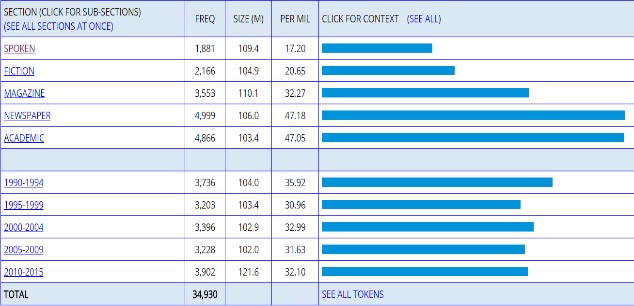
\includegraphics[width=\textwidth]{figures/Othercycles-COCA.jpg}
%\caption{\textit{Failed to} and a verb in COCA.}
%\label{fig:oth-COCA}
%\end{figure}
%
\begin{table}\begin{small}
\caption{\textit{Failed to} and a verb in COCA.}
\label{tab:oth-COCA}
\begin{tabularx}{\textwidth}[]{l r r r l}
\lsptoprule
Section     &Freq   &Size (M)   &Per Mil    &   \\
\midrule
spoken      &1,881  &109.4      &17.20      &\cocabar{17.20}   \\
fiction     &2,166  &104.9      &20.65      &\cocabar{20.65}    \\
magazine    &3,553  &110.1      &32.27      &\cocabar{32.27}    \\
newspaper   &4,999  &106.0      &47.18      &\cocabar{47.18}    \\
academic    &4,866  &103.4      &47.05      &\cocabar{47.05}    \\
\midrule
1990--1994  &3,736  &104.0      &35.92      &\cocabar{35.92}    \\
1995--1999  &3,203  &103.4      &30.96      &\cocabar{30.96}    \\
2000--2004  &3,396  &102.9      &32.99      &\cocabar{32.99}    \\
2005--2009  &3,228  &102.0      &31.63      &\cocabar{31.63}    \\
2010--2015  &3,902  &121.6      &32.10      &\cocabar{32.10}    \\
\midrule
Total       &34,930 &           &           &                   \\
\lspbottomrule
\end{tabularx}\end{small}\end{table}

As several people have mentioned to me, this verb is so negative (in
American culture) that it probably won't catch on. Its use in the British
National Corpus (e.g. in spoken) is even lower though not in the written
registers. Other negative verbs, e.g. \textit{lack}, don't show this
either, however.

In this subsection, negative verbs have been shown to be the source for the
NEC.

\subsection{Non-verbal nature}\label{sec:oth-3.2}

Some scholars have tried to unify the NEC and the JC,  
e.g. \textcitetv{chapters/Intertwining-Auwera-Krasnoukhova-Vossen}. In addition, Veselinova's definition of the NEC
includes reanalyzing non-verbal material from existential constructions.
The relevant example that \citet[136]{Veselinova2013} mentions is from
Ket. In this section, I argue against including these into the NEC. I'll
first discuss the adverb\slash noun sources followed by the existential
pro-form.

The JC has traditionally been seen as a nominal cycle because its source is
a negative noun, such as \textit{nan wuht} `no thing' in
\REF{ex:other-OE-understand}, or a minimizer, such as French \textit{pas}
`step'. These nouns can be reanalyzed as adverbs in
\REF{ex:other-OE-occupied}. 
%
\begin{exe}\ex Old English \label{ex:other-OE-understand}\il{English}\\
    \gll forþæmþe hie hiora \textbf{nan wuht} ongietan \textbf{ne} meahton
    \\ 
  because they their {no thing} understand not could \\
    \glt `because they couldn't understand anything'
(Alfred, \textit{Pastoral Care} 4.12 Cotton, \citealt[81]{Gelderen2004})
    \ex Old English \label{ex:other-OE-occupied}\il{English}\\
    \gll Næron 3e \textbf{noht} æmetti3e, ðeah ge wel ne dyden \\
not-were you not unoccupied though you well not did \\
    \glt `You were not unoccupied, though you did not do well.' 
(OED, Alfred, \textit{Pastoral Care} 207.20 Cotton, \citealt[82]{Gelderen2004})
    \end{exe}
%
The JC typically renews the negative element \textit{ne} by a new noun \textit{nawhiht} whereas the NEC replaces the verb that has become part of the negative.

The example that has been used to show that non-verbal material from
existential constructions is reanalyzed is a solitary one from Ket\il{Ket}.
In Ket, \textit{bən's’aŋ} `there are no' derives from the negative
\textit{bənj} and \textit{us'aŋ} `there', according to \textcite[136, but
without a reference]{Veselinova2015} and this would use non-verbal parts
of the construction. The Ket dictionary \parencite{KotorovaNefedov2015}
confirms \textit{bən} as negative (\citeyear[135]{KotorovaNefedov2015}),
\textit{bənsaŋ} `there are no' (\citeyear[136]{KotorovaNefedov2015}), and
\textit{usaŋ\slash usam} as `there are'
(\citeyear[415]{KotorovaNefedov2015}). The existential particles
\textit{bənsaŋ} and \textit{usaŋ\slash usam} do not agree with the subject
or mark tense and are also used to mark locative or possessives, as shown
in \REF{ex:other-ket-rifle}.
%
\begin{exe}\ex Ket \label{ex:other-ket-rifle}\il{Ket}\\
    \gll {\'ɔ}pdaŋ   b{\'ɔ}gdɔm    \textbf{b{\'ʌ}nsaŋ} \\
father  rifle    not.exist \\
    \glt `Father has no rifle.' (\citealt[65]{KotorovaNefedov2015}, but gloss adjusted)
    \end{exe}
%
Using the dictionary information, it is possible to regard
\textit{usaŋ\slash usam} `there are' in Ket\il{Ket} as a copula (possibly originating
from a demonstrative like Arabic) and then \textit{bənsaŋ} is the
combination of a negative and a copula, quite typical for the NEC.

Concluding, I have shown an interaction between the Givon Cycle and the NEC
in \sectref{sec:oth-3.1} and have shown in \sectref{sec:oth-3.2} that the
instance where a non-verbal part of the existential seems to participate in
the NEC is just a negative form of the copula. The use of non-verbal
material in the NEC is very rare.  For instance, in their compilation of
typical grammaticalizations, \citet[199--206]{HeineKuteva2002} mention a
development where a locative develops into an existential (e.g.
Sranan\il{Sranan} \textit{de} `to be' from the locative \textit{there}) but
this is part of the copula cycle \parencite{Gelderen2015}. This locative,
having become a copula, can of course be input to a NEC, just like
demonstratives that have been reanalyzed as copulas.

\section{Doubling}\label{sec:oth-4}

A last question concerns another difference between the JC and the NEC,
namely that doubling is typical for JC but not for the NEC. This follows
from the ways the cycles procede: the NEC has a negative with an
existential (or copula or auxiliary) serve as a sentential negative and
there is therefore no doubling of the negative but rather of the copula. In
contrast, the JC is about pragmatic strengthening by a second negative and
therefore doubling is typical. In this section, I discuss two possible
counterexamples to the claim that doubling the negative is not typical of
the NEC.

\citet[10]{Croft1991} mentions the case of Wintu\il{Wintu} where the
negative existential \textit{ˁelew} is reinforcing the regular negative
\textit{-mina} in \REF{ex:other-wintu-go}. 

\begin{exe}\ex Wintu \label{ex:other-wintu-go}\il{Wintu}\\
    \gll \textbf{ˁelew}-be:sken    hara:-wer-\textbf{mina} \\
  \textsc{neg.ex}-you.\textsc{ipfv}  go-\textsc{fut-neg} \\
    \glt `You were not supposed to go.' \citep[198]{Pitkin1984}
    \end{exe}
%
The morpheme -\textit{mina} derives most likely from the verb root
\textit{min} `to not exist'
\parencites[361]{Schlichter1981}[121]{Pitkin1984} and is also related to
\textit{minel} `be dead; die' \citep[146]{Schlichter1981}.
\citet[311]{Schlichter1981} refers to \textit{ˁelew} as a negative
auxiliary preverb so this language renews its negative auxiliaries with
negative verbs (the Givón Cycle). 

It is not clear from Croft, Schlichter, or Pitkin what the process was for
adding \textit{ˁelew}\il{Wintu} in \REF{ex:other-wintu-go}. The negative auxiliary
\textit{ˁelew} is reconstructed from a demonstrative *ˁE and stative *l or
future *le and a suffix *w \citep[164]{Pitkin1984}. The examples of a
solitary \textit{ˁelew} given by \citet[198]{Pitkin1984} are optative or
imperative prefixes, as in \REF{ex:other-wintu-venture}, or on its own, as in
\REF{ex:other-wintu-coyote}.

\begin{exe}\ex Wintu \label{ex:other-wintu-venture}\il{Wintu}\\
    \gll \textbf{ˁelew}-war \\
\textsc{neg.ex}-go \\
    \glt `don't venture' \citep[198]{Pitkin1984}
    \ex \label{ex:other-wintu-coyote}\il{Wintu}
    \gll sedet  \textbf{ˁelew}  k̓iyemti·m \\
coyote  not  old.man.speak \\
    \glt `Coyote never speaks wisely.' \citep[269]{Pitkin1984}
    \end{exe}
%
This means that \textit{ˁelew} can be analyzed in Wintu\il{Wintu} as a
copula in origin that became used with other negatives. There is no
evidence that there was ever a stage with two negative existentials in this
language but further work is needed.

\citet{chapters/Chadic-Butters} mentions some NEC cases from Chadic that suggest
doubling of the negative, based in part on \citet{Shay2008} who, in her
grammar of South Giziga, mentions an existential consisting of two
negatives, namely \REF{ex:other-giziga-angry}. The verb \textit{(á)n} only occurs in
negative clauses and is therefore glossed as `be.\textsc{neg}'.
%
\begin{exe}\ex South Giziga \label{ex:other-giziga-angry}\il{South
Giziga}\\
    \gll kà  \textbf{n}  \textbf{tá}  sà  jí  mèvèl      \\
2  be.\textsc{neg}  \textsc{neg}  \textsc{fut}  catch  liver \\
    \glt
‘You will not be angry.' (\citealt{Shay2008}, chapter 13)
    \end{exe}
%
Shay mentions that a ``likely source for the negative existential predicate
is a verb \textit{n}V meaning `be'' supported by Lukas' (\citeyear[151]{Lukas1970}) report of a
North Giziga -\textit{naŋ} `to be'. I therefore think this is not a case of
doubling but just of an existential being used with a negative, i.e. stage
B.

\section{Structural characteristics of the NEC, JC, and the Givón
Cycle}\label{sec:oth-5}

In this paper, I have argued that there are three negative cycles, NEC, JC, and the Givón Cycle, with the NEC interacting with Givón's and the Copula Cycles (which renew the existential lost in the NEC). In this section, I will provide formal descriptions of each of these cycles showing that they differ.

For ease of exposition, I provide English morphemes for the NEC. A
possible NEC may go from having the same negative with a full verb and an
existential in \REF{ex:other-phases-a} to \REF{ex:other-phases-b} where the negative
and existential are fused because the existential moves to the Neg head
on its way to T. Finally, in \REF{ex:other-phases-c}, the reanalyzed negative
serves both existential and standard negatives and an optional new copula
may appear.
\pagebreak


%     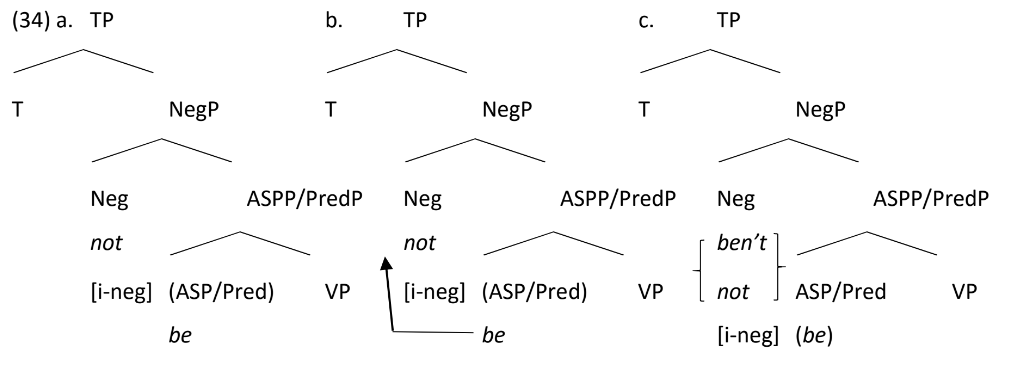
\includegraphics[width=\textwidth]{figures/gelderen_ex34.png}

\ea\label{ex:other-phases}
\begin{multicols}{2}\raggedcolumns
\ea\label{ex:other-phases-a}
    \begin{forest}
      [TP
        [T]
        [NegP
            [{Neg\\\textit{not}\\{}[i-neg]}]
            [ASPP/PredP
                [{(ASP/Pred)\\\textit{be}}]
                [VP]
            ]
        ]
      ]
    \end{forest}\columnbreak
\ex\label{ex:other-phases-b}
    \begin{forest}
      [TP
        [T]
        [NegP
            [{Neg\\\textit{not}\\{}[i-neg]}, name=neg]
            [ASPP/PredP
                [{(ASP/Pred)\\\textit{be}},name=be]
                [VP]
            ]
        ]
      ]
      \draw[->] (be) to[out=south west,in=south west] (neg);
    \end{forest}
\z
\end{multicols}
\begin{xlist}
\setcounter{xnumii}{2}
\ex\label{ex:other-phases-c}
    \begin{forest}
      [TP
        [T]
        [NegP
            [{Neg\\$\left\{\begin{tabular}{@{}c@{}}\itshape ben't\\\itshape not\end{tabular}\right\} $\\{}[i-neg]}]
            [ASPP/PredP
                [{(ASP/Pred)\\(\textit{be}\/)}]
                [VP]
            ]
        ]
      ]
    \end{forest}
\end{xlist}
\z

Because the NEC can have a copula as its source, the Pred(icate) P(hrase)
is used in \REF{ex:other-phases}; the ASP(ect) P(hrase) is needed for stages of
the NEC that are aspectually restricted, as in Chinese.

The trigger for this cycle is that copula verbs can be zero and the child
reanalyzes the copula as part of the negative. For instance,
\citet{Becker2000} shows that young children omit the copula especially
when the predicate expresses a temporary property (with an aspectual
representation).\largerpage[2]

Turning to the JC, these changes don't single out a special kind of verb;
this cycle typically takes a negative or indefinite noun to renew a
negative head. \citet[139]{Meillet1912} writes that what provokes the start
of the (negative) cycle is the need to speak forcefully (``le besoin de
parler avec force''). \citet{KiparskyCondoravdi2006}, in examining
Jespersen's Cycle in Greek, find no evidence for phonetic weakening and
similarly suggest pragmatic and semantic reasons. A simple negative cannot
be emphatic; in order for a negative to be emphatic, it needs to be
reinforced, e.g. by a minimizer. Adapting ideas from \citet{Dahl2001}, they
argue that, when emphatic negatives are overused, their semantic impact
weakens and they become the regular negative and a new emphatic will
appear. I have provided these changes in \REF{ex:other-more-phases}. In
\REF{ex:other-more-phases-a}, there is one negative, represented by Old English
\textit{ne}; in \REF{ex:other-more-phases-b}, there is a second negative which, because
it is agreeing with the negative features in the NegP, moves to the Spec of
NegP and then the original negative is reinterpreted as head.

\ea
\label{ex:other-more-phases}
\setlength{\columnsep}{-10pt}
\begin{multicols}{2}\raggedcolumns
%     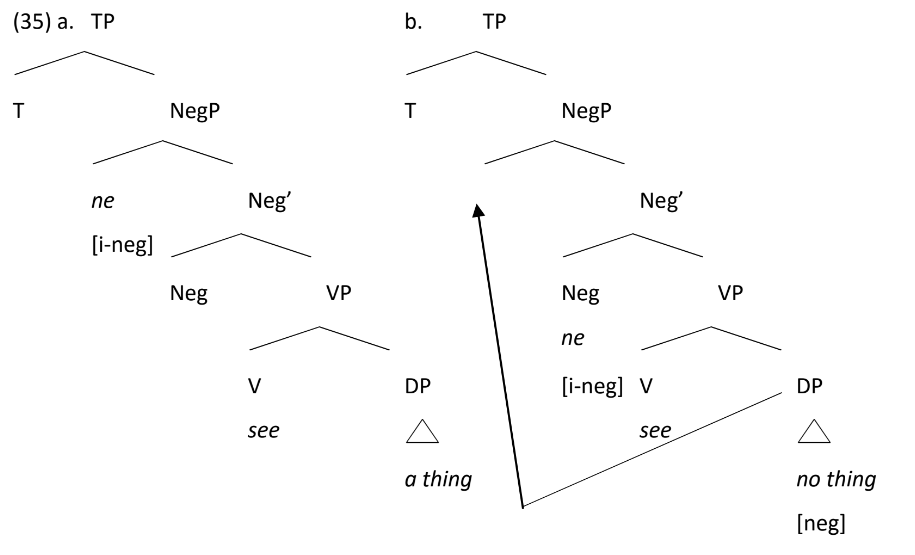
\includegraphics[width=\textwidth]{figures/gelderen_ex35.png}
\ea\label{ex:other-more-phases-a}
    \begin{forest}
      [TP
        [T]
        [NegP
            [{\textit{ne}\\{}[i-neg]}]
            [Neg$'$
                [Neg]
                [VP
                    [{V\\\textit{see}}]
                    [DP
                        [\textit{a thing}, roof]
                    ]
                ]
            ]
        ]
      ]
    \end{forest}\columnbreak
\ex\label{ex:other-more-phases-b}
    \begin{forest}
      [TP
        [T]
        [NegP
            [~, name=empty]
            [Neg$'$
                [{Neg\\\textit{ne}\\{}[i-neg]}]
                [VP
                    [{V\\\textit{see}}]
                    [DP
                        [{\textit{no thing}\\{}[neg]}, roof, name=DP]
                    ]
                ]
            ]
        ]
      ]
      \draw[->] (DP) to[bend left=90] (empty);
    \end{forest}
\z
\end{multicols}
\z


Finally, the negative features of the DP are reanalyzed as the grammatical
negative features and housed in the specifier of the NegP and we are back
to \REF{ex:other-more-phases-a}.

The Givón Cycle involves the reanalysis of a verb into an aspect marker into
a negative. This could be represented as a change from
\REF{ex:other-even-more-phases-a} to
\REF{ex:other-even-more-phases-b}, with Chinese as the example language.

\noindent\parbox{\textwidth}{\ea
    \label{ex:other-even-more-phases}
%     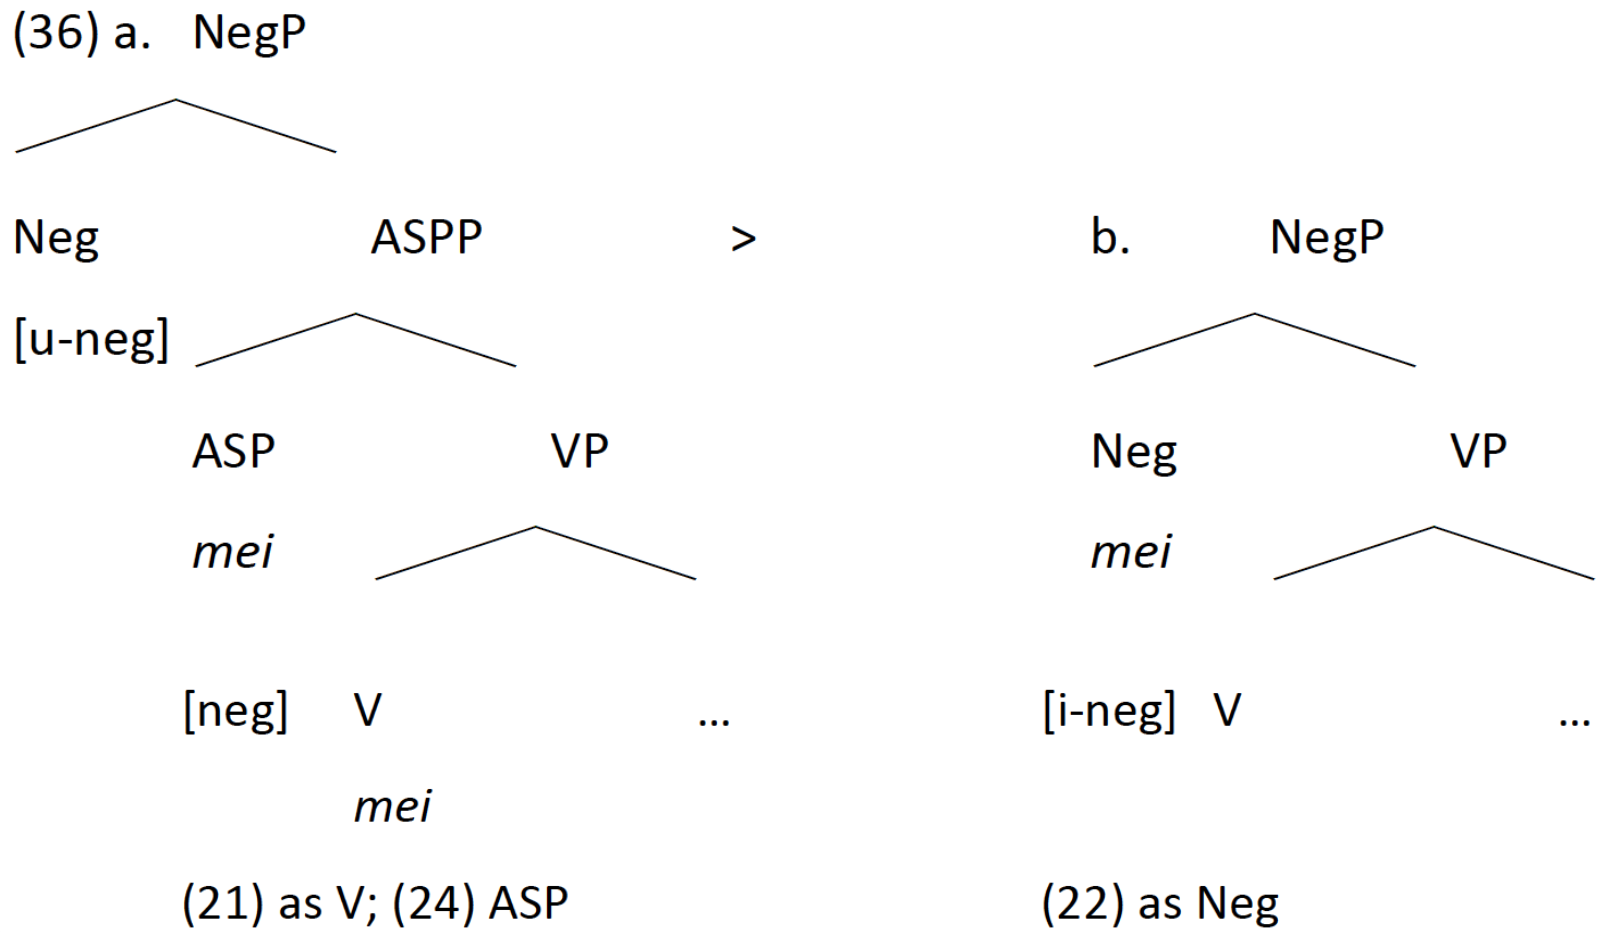
\includegraphics[width=0.5\textwidth]{figures/gelderen_ex36.png}
\begin{multicols}{2}\raggedcolumns
\ea \label{ex:other-even-more-phases-a}
\begin{forest}
      [NegP
        [{Neg\\{}[u-neg]}]
        [ASPP
            [{Asp\\\textit{mei}}]
            [VP
                [{V\\\textit{mei}}]
                [\dots]
            ]
        ]
      ]
    \end{forest}\columnbreak
\ex \label{ex:other-even-more-phases-b}
    \begin{forest}
      [NegP
        [{Neg\\\textit{mei}\\{}[i-neg]}]
            [VP
                [V]
                [\dots]
            ]
        ]
    \end{forest}
\z\end{multicols}
\z}


The reason English\il{English} \textit{failed to} in \REF{ex:other-even-more-phases-b}
shows no inclination to take over as [i-neg] is related to English verbs
having other features, e.g. tense and agreement and not being reanalyzable
as a simple negative. The same hold for the NEC because a negative and a
verb are hard to reanalyze as verb if there are too many agreement and
other features involved. The JC doesn't encounter these obstacles.

\section{Conclusions}\label{sec:oth-6}

In this paper, I argue in favor of seeing the NEC as a verbal cycle that
combines a `be'-like verb with a negative and then renews the
existential\slash copular verb. The JC is a non-verbal cycle, with
renewals originating in nouns and adverbs. Both the NEC and the Givón Cycle
rely on verbs for their renewal and work best when these verbs don't have
too many other features; JC is not affected by these verbal features. 

\section*{Acknowledgements}\label{sec:oth-acknowledgements}

Some ideas in this paper are based on chapters 4 and 8 in
\textcite{Gelderen2011}. I thank Mekhlid Alsaeedi, Cherry Lam, and Ljuba
Veselinova for comments.


\section*{List of languages}

\begin{tabularx}{.5\textwidth}{@{}lQ}
Ahtna           &aht\\
Arabic          &arb \\
Bearlake        &scs \\
Cantonese       &yue \\
Carrier         &crx \\
Chinese         &chi \\
Chipewyan\slash Dëne S\k{u}łiné  &chp\\
Egyptian Arabic    &arz\\
English         &eng\\
Estonian        &est \\
Finnish         &fin\\
\end{tabularx}\begin{tabularx}{.5\textwidth}{lQ@{}}
Hindi           &hin\\
Ket             &ket\\
Kwadacha        &sek\\
Marathi         &mar\\
Skolt Saami     &sms\\
South Giziga    &giz\\
Southern Saami    &sma\\
Tlingit         &tli\\
Urdu            &urd\\
Wintu           &wnw\\
\\
\end{tabularx}

\section*{Abbreviations}

\begin{tabularx}{.5\textwidth}{@{}l l}
\textsc{asp}    &aspect\\
\textsc{conneg} &negative participle\\ 
\textsc{cop}    &copula\\
\textsc{ex}     &affirmative existential\\
\textsc{emph}    &emphatic\\
\textsc{fut}    &future\\
\textsc{jc}     &Jespersen Cycle\\ 
\textsc{ipfv}    &imperfective\\
\textsc{irr}    &irrealis\\
\end{tabularx}\begin{tabularx}{.5\textwidth}{l l@{}}
\textsc{nec}    &Negative Existential Cycle\\ 
\textsc{neg}    &negative\\ 
\textsc{om}    &object marker\\
\textsc{pfv}   &perfective\\
\textsc{pred}   &predicate\\
\textsc{prog}   &progressive\\
\textsc{prs}   &present\\
\textsc{pst}   &past\\
\textsc{prt}    &particle\\
\end{tabularx}


\section*{Sources}

British National Corpus (BNC)\\
Corpus of Contemporary American English (COCA)\\
Corpus of Historical American English (COHA)\\

{\sloppy\printbibliography[heading=subbibliography]}
\end{document}
